\chapter{Конструкторская часть}
В этом разделе будут приведены схемы алгоритмов и вычисления трудоемкости данных алгоритмов.
\section{Разработка алгоритмов}

На рисунках \ref{fig:worker}, \ref{fig:dispatcher}, \ref{fig:follow} представлены схемы алгоритмов рабочего потока, потока диспетчера, и последовательного алгоритма обратной трассировки лучей.
%поправить циклы добавить надпись конца цикла
\begin{figure}[H]
	\centering
	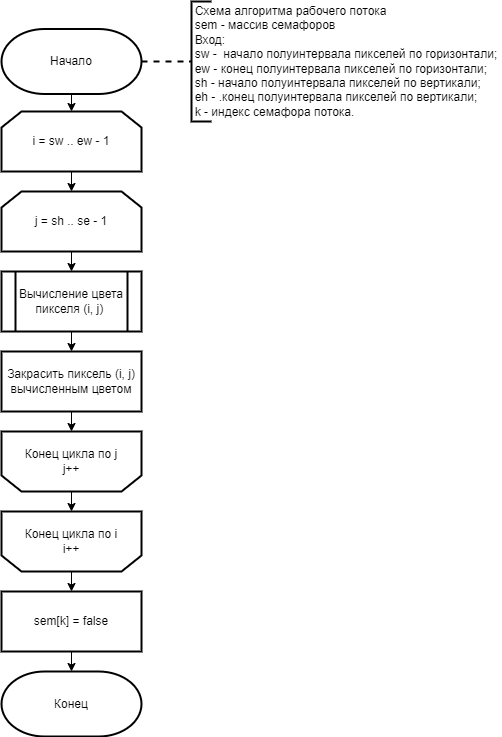
\includegraphics[width=0.7\linewidth]{inc/img/worker}
	\caption{Схема алгоритма рабочего потока}
	\label{fig:worker}
\end{figure}
\begin{figure}[H]
	\centering
	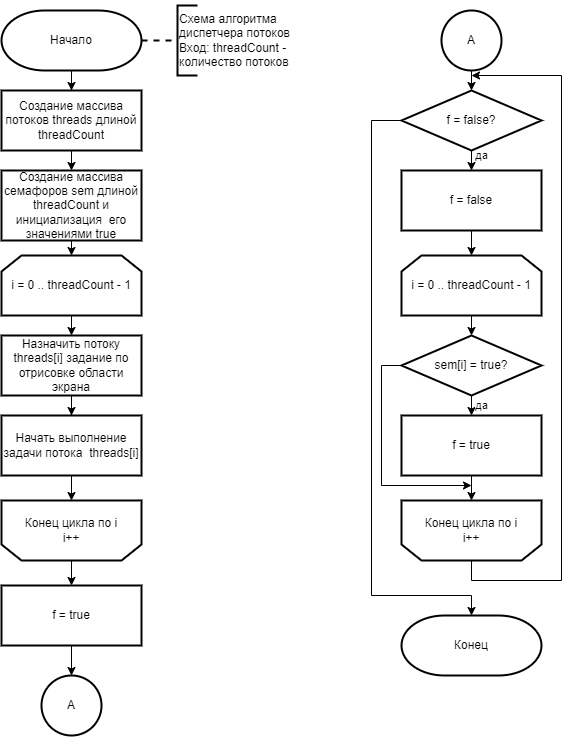
\includegraphics[width=0.7\linewidth]{inc/img/dispatcher}
	\caption{Схема алгоритма потока диспетчера}
	\label{fig:dispatcher}
\end{figure}
\captionsetup{justification=centering,singlelinecheck=true}
\begin{figure}[H]
	\centering
	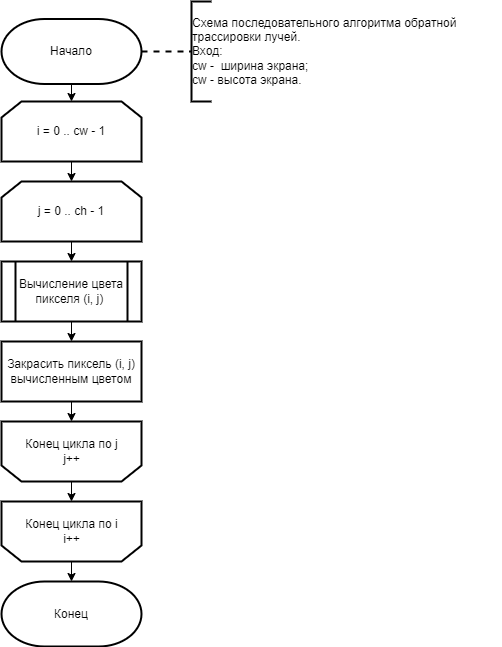
\includegraphics[width=0.7\linewidth]{inc/img/follow}
	\caption{Схема последовательного алгоритма обратной трассировки лучей}
	\label{fig:follow}
\end{figure}



\section*{Вывод}

Были разработаны схемы трех алгоритмов, а именно алгоритмов для рабочего потока, для потока-диспетчера, и последовательного алгоритма обратной трассировки лучей.


